\documentclass[xcolor={table}]{beamer}
%\usetheme{singapore}
\usepackage{bm}
\usepackage{listings,verbatim}
\usepackage{fancyvrb,tikz,color,xcolor,colortbl}
\usepackage{hyperref,booktabs,tabularx,float}
\usepackage{multirow}
%\usepackage[table]{xcolor}
%\usepackage{verbatim}
% \usepackage{array}
%\lstloadlanguages{R}
%\lstset{ language=R, basicstyle=\scriptsize\ttfamily, commentstyle=\ttfamily\color{gray}, numbers=left, numberstyle=\ttfamily\color{gray}\footnotesize, stepnumber=1, numbersep=5pt, backgroundcolor=\color{white}, showspaces=false, showstringspaces=false, showtabs=false, frame=single, tabsize=2, captionpos=b, breaklines=true, breakatwhitespace=false, escapeinside={}, keywordstyle={}, morekeywords={} }\renewcommand{\P}{\mathcal{P}}
%\newcommand{\bt}{\pmb{\theta}}
%\newcommand{\bG}{\pmb{\Gamma}}
\newcommand{\p}{\pause}
\definecolor{Grey}{rgb}{0.95,0.95,0.95}
\definecolor{lred}{rgb}{1,.8,.8}
\definecolor{lblue}{rgb}{.8,.8,1}
\newcommand{\pitem}{\pause \item}
\newenvironment{graytext}{\color{gray}}{\ignorespacesafterend}

\newcommand\independent{\protect\mathpalette{\protect\independenT}{\perp}}
\def\independenT#1#2{\mathrel{\rlap{$#1#2$}\mkern2mu{#1#2}}}

\definecolor{umassblue}{RGB}{51,51,153}
\definecolor{umassgreen}{RGB}{0,102,102}
%\definecolor{blue}{RGB}{51,51,153}
\definecolor{bblue}{RGB}{0,0,255}
\definecolor{red}{RGB}{153,0,51}

\newcommand\verbbf[1]{\textcolor[RGB]{51,51,153}{\textbf{$\blacksquare$ #1}}}
\newcommand\verbrf[1]{\textcolor[RGB]{153,0,51}{\textbf{$\blacksquare$ #1}}}

\newcommand{\N}{\mathcal{N}}
\newcommand{\Y}{\bm{\mathcal{Y}}} 

\usefonttheme{serif}

\newenvironment{changemargin}[2]{%
  \begin{list}{}{%
    \setlength{\topsep}{0pt}%
    \setlength{\leftmargin}{#1}%
    \setlength{\rightmargin}{#2}%
    \setlength{\listparindent}{\parindent}%
    \setlength{\itemindent}{\parindent}%
    \setlength{\parsep}{\parskip}%
  }%
  \item[]}{\end{list}} 

%
\title{\LARGE Reading between the Emails: Gendered Patterns of Communication in Local Government}
%
\definecolor{umassred}{HTML}{8C2633}
\setbeamercolor{structure}{fg=umassblue} 
\author{\large\textbf{Matthew J. Denny}}

%\affil[1]{University of Massachusetts Amherst}
%\affil[2]{University of Connecticut}

\institute{\large Penn State University --- 
 \texttt{mdenny@psu.edu}\\
 \color{blue}\texttt{www.mjdenny.com}\\ 
 \texttt{@MatthewJDenny}
}

\date{Collaborators: James ben Aaron, Hanna Wallach,\\ Bruce A. Desmarais}
\begin{document}


\begin{frame}
  \titlepage
\end{frame}


\begin{frame}\frametitle{Gender and Communication in Local Government}
	\LARGE
	\begin{itemize}
		\item Gender bias in organizations.
		\vspace*{.3in}
		\item How does gender shape communication?
		\vspace*{.3in}
		\item Differences across domains?
		\vspace*{.3in}
		\item Relation to previous findings?
	\end{itemize}
\end{frame}


\begin{frame}\frametitle{Challenges and Opportunities}
	\LARGE
	\begin{itemize}
		\item Observational and self report data.
		\vspace*{.15in}
		\begin{itemize}
			\LARGE
			\item Restricted in scope. Biased? 
		\end{itemize}
		\vspace*{.15in}
		\item Electronic communication data.
		\vspace*{.15in}
		\begin{itemize}
			\LARGE
			\item Primary source, day-to-day.
			\vspace*{.15in}
			\item Public records laws.
		\end{itemize}
		\vspace*{.15in}
		\item Study micro-level interactions.
	\end{itemize}
	
\end{frame}

\begin{frame}\frametitle{}
	\begin{center}
		\Huge\textbf{Public Domain Email Data}
	\end{center}
\end{frame}

\begin{frame}\frametitle{County Government Email Data}
	\Large
	\begin{itemize}
		\item Public records requests.
		\vspace*{.1in}
		\item Department manager email data from 17 North Carolina Counties.
		\vspace*{.1in}
		\item 500,000 emails, 17,000 between managers.
		\vspace*{.1in}
	\end{itemize}
	\centering
	
\includegraphics[width=0.95\textwidth]{images/County_Map.pdf}
\end{frame}


\begin{frame}\frametitle{The Data}
	\Large
\begin{changemargin}{-1cm}{ -1cm}	
	  \centering
	  \vspace*{-.3in}
	  \centering
	  \begin{tabular}{lrrrr}
	    \toprule
	    & \multicolumn{2}{c}{Manager Gender} & \\
	    \cmidrule{2-3}
	    County & Male & Female & \# Emails  \\
	    \midrule
	    Alexander & 12 & 9 & 907   \\
	    Caldwell & 12 & 8 & 121     \\
	    Chowan & 12 & 11 & 2,027   \\
	    Columbus & 14 & 10 & 920   \\
	    Dare & 15 & 12 & 2,247    \\
	    Duplin & 13 & 14 & 1,914    \\
	    % Hoke & 13 & 11 & 1,106  \\
  % 	    Jackson & 18 & 6 & 1,499    \\
		\vdots & \vdots & \vdots & \vdots \\
	    % Lenoir & 15 & 5 & 560  \\
% 	    Lincoln & 15 & 7 & 573   \\
% 	    McDowell & 12 & 5 & 326   \\
% 	    Montgomery & 8 & 10 & 680   \\
% 	    Nash & 11 & 8 & 1,147  \\
	    % Person & 12 & 9 & 1,491   \\
	    Transylvania & 16 & 4 & 1,857  \\
	    Vance & 10 & 8 & 185   \\
	    Wilkes & 15 & 2 & 303   \\
	    \midrule
	    Total & 223 & 139 & 17,863 \\
	    \bottomrule
	  \end{tabular}

\end{changemargin}

\end{frame}

\begin{frame}\frametitle{}
	\begin{center}
		\Huge\textbf{Descriptive Analysis}
	\end{center}
\end{frame}

\begin{frame}\frametitle{Aggregate Patterns}
	
	\begin{changemargin}{-1cm}{ -1cm}
	\Large
	\centering
    \begin{tabular}{lrrr}
      \toprule
      & \multicolumn{2}{c}{Manager Gender} \\
      \cmidrule{2-3}
      & Male & Female  \\
      \midrule
      Average \# emails sent & 48.3 & 51 \\
      Average \# recipients per email sent & 1.45 & 1.43 \\
      \midrule
      Average \# emails received & 70.8 & 71.6 \\
      \bottomrule
    \end{tabular}
	\end{changemargin} 
	
	\bigskip
	\centering
	\Large
	
	
	\begin{itemize}
		\item No evidence for gender bias in aggregate.
		\vspace*{.1in}
		\item Mild gender-heterophily.
	\end{itemize}
	
	% \begin{tabular}{rlrrr}
% 	  \toprule
% 		 && \multicolumn{2}{c}{Recipient} \\
% 		\cmidrule{3-4}
% 	& & Male & Female & Total  \\
% 		 \midrule
% 		\multirow{2}{*}{Sender} & Male & 7,299 & 6,286 & 13,585 \\
% 	& Female & 5,325 & 3,510 & 8,835 \\
% 	\midrule
% 		 & Total & 12,624 & 9,796 & \\
% 		\bottomrule
% 		\end{tabular}
		
\end{frame}


\begin{frame}\frametitle{Individual Department Gender Breakdown}
	
	\begin{changemargin}{-1cm}{ -1cm}
		\Large
    \centering
	\setlength{\tabcolsep}{3pt}
	  \begin{tabular}{rrrrrrrrrrrrrrrrrrrrrrrr}
	    \toprule
	
		   & \cellcolor{lred} \rotatebox{90}{Emergency} & \cellcolor{lred}\rotatebox{90}{Manager} & \cellcolor{lblue}\rotatebox{90}{HR} & \cellcolor{lblue}\rotatebox{90}{Finance} & \rotatebox{90}{IT} & \cellcolor{lblue}\rotatebox{90}{Health} & \rotatebox{90}{Plan/Dev} & \cellcolor{lred}\rotatebox{90}{Util/Waste} & \rotatebox{90}{Tax} & \rotatebox{90}{Parks/Rec} & \rotatebox{90}{Soc\_Serv} & \rotatebox{90}{Transport} & \rotatebox{90}{Info} & \rotatebox{90}{Misc} & \rotatebox{90}{Inspections} \\ % & \rotatebox{90}{Maintenance} & \rotatebox{90}{Library} & \rotatebox{90}{Veterans} & \rotatebox{90}{Seniors} & \rotatebox{90}{Animal}  \\ 
		     \midrule
		   Male & \cellcolor{lred}29 & \cellcolor{lred}15 & \cellcolor{lblue}3 & \cellcolor{lblue}5 & 11 & \cellcolor{lblue}6 & 17 & \cellcolor{lred}15 & 11 & 9 & 8 & 8 & 2 & 5 & 13 \\  %& 5 & 3 & 5 & 2 & 9  \\ 
		     Female & \cellcolor{lred}3 & \cellcolor{lred}2 & \cellcolor{lblue}12 & \cellcolor{lblue}12 & 2 & \cellcolor{lblue}11 & 6 & \cellcolor{lred}2 & 7 & 5 & 10 & 1 & 6 & 2 & 3 \\% & 1 & 8 & 7 & 6 & 3  \\ 
			 \midrule
		     Total & \cellcolor{lred}32 & \cellcolor{lred}17 & \cellcolor{lblue}15 & \cellcolor{lblue}17 & 13 & \cellcolor{lblue}17 & 23 & \cellcolor{lred}17 & 18 & 14 & 18 & 9 & 8 & 7 & 16 \\ %& 6 & 11 & 12 & 8 & 12 \\
	    \bottomrule
	    \end{tabular}
	\setlength{\tabcolsep}{6pt}
\bigskip
\bigskip

\begin{tabular}{l}
	\cellcolor{lred} Male dominated positions\\
	\cellcolor{lblue} Female dominated positions 
\end{tabular}
\end{changemargin} 
\end{frame}

\begin{frame}\frametitle{}
	\begin{center}
		\Huge\textbf{Department Affiliation as Domain}
	\end{center}
\end{frame}


\begin{frame}\frametitle{Female-Centric Dyads}
	\centering
	\Large
	\begin{tabular}{l}
	  \toprule
	FF $>$ FM $>$ MF $>$ MM  \\
	\hline
	  HR \& Health  \\ 
	  HR \& Information Technology  \\ 
	  HR \& County Manager  \\ 
	  Planning \& HR \\ 
	  Register of Deeds \& HR  \\ 
	  Parks and Recreation \& HR  \\ 
	  Finance \& HR  \\ 
	  Finance \& Parks and Recreation  \\ 
	  Social Services \& HR  \\ 
	  Solid Waste and Recycling \& HR  \\ 
	  Tax Administrator \& HR  \\ 
	   \bottomrule
	\end{tabular}
	
	
	
	
\end{frame}


\begin{frame}\frametitle{Male-Centric Dyads}
	\centering
	\Large
	\begin{tabular}{l}
	  \toprule
	  MM $>$ FM $>$ MF $>$ FF \\ 
	  \midrule
	  Planning \& Information Technology \\ 
	  Solid Waste and Recycling \& Health \\ 
	  Sheriff \& Health  \\ 
	  Tax Administrator \& Planning  \\ 
	  Tax Administrator \& Social Services  \\ 
	  Inspections \& Tax Administrator  \\ 
	  Animal Control \& Finance   \\ 
	  Environment \& Health  \\ 
	  Environment \& Solid Waste and Recycling  \\  
	   \bottomrule
	\end{tabular}
	
	
	
	
\end{frame}

\begin{frame}\frametitle{}
	\begin{center}
		\Huge\textbf{Email Content as Domain}
	\end{center}
\end{frame}


\begin{frame}\frametitle{A Generative Model for Email Data}
	\begin{changemargin}{-1cm}{ -1cm}
    \centering
	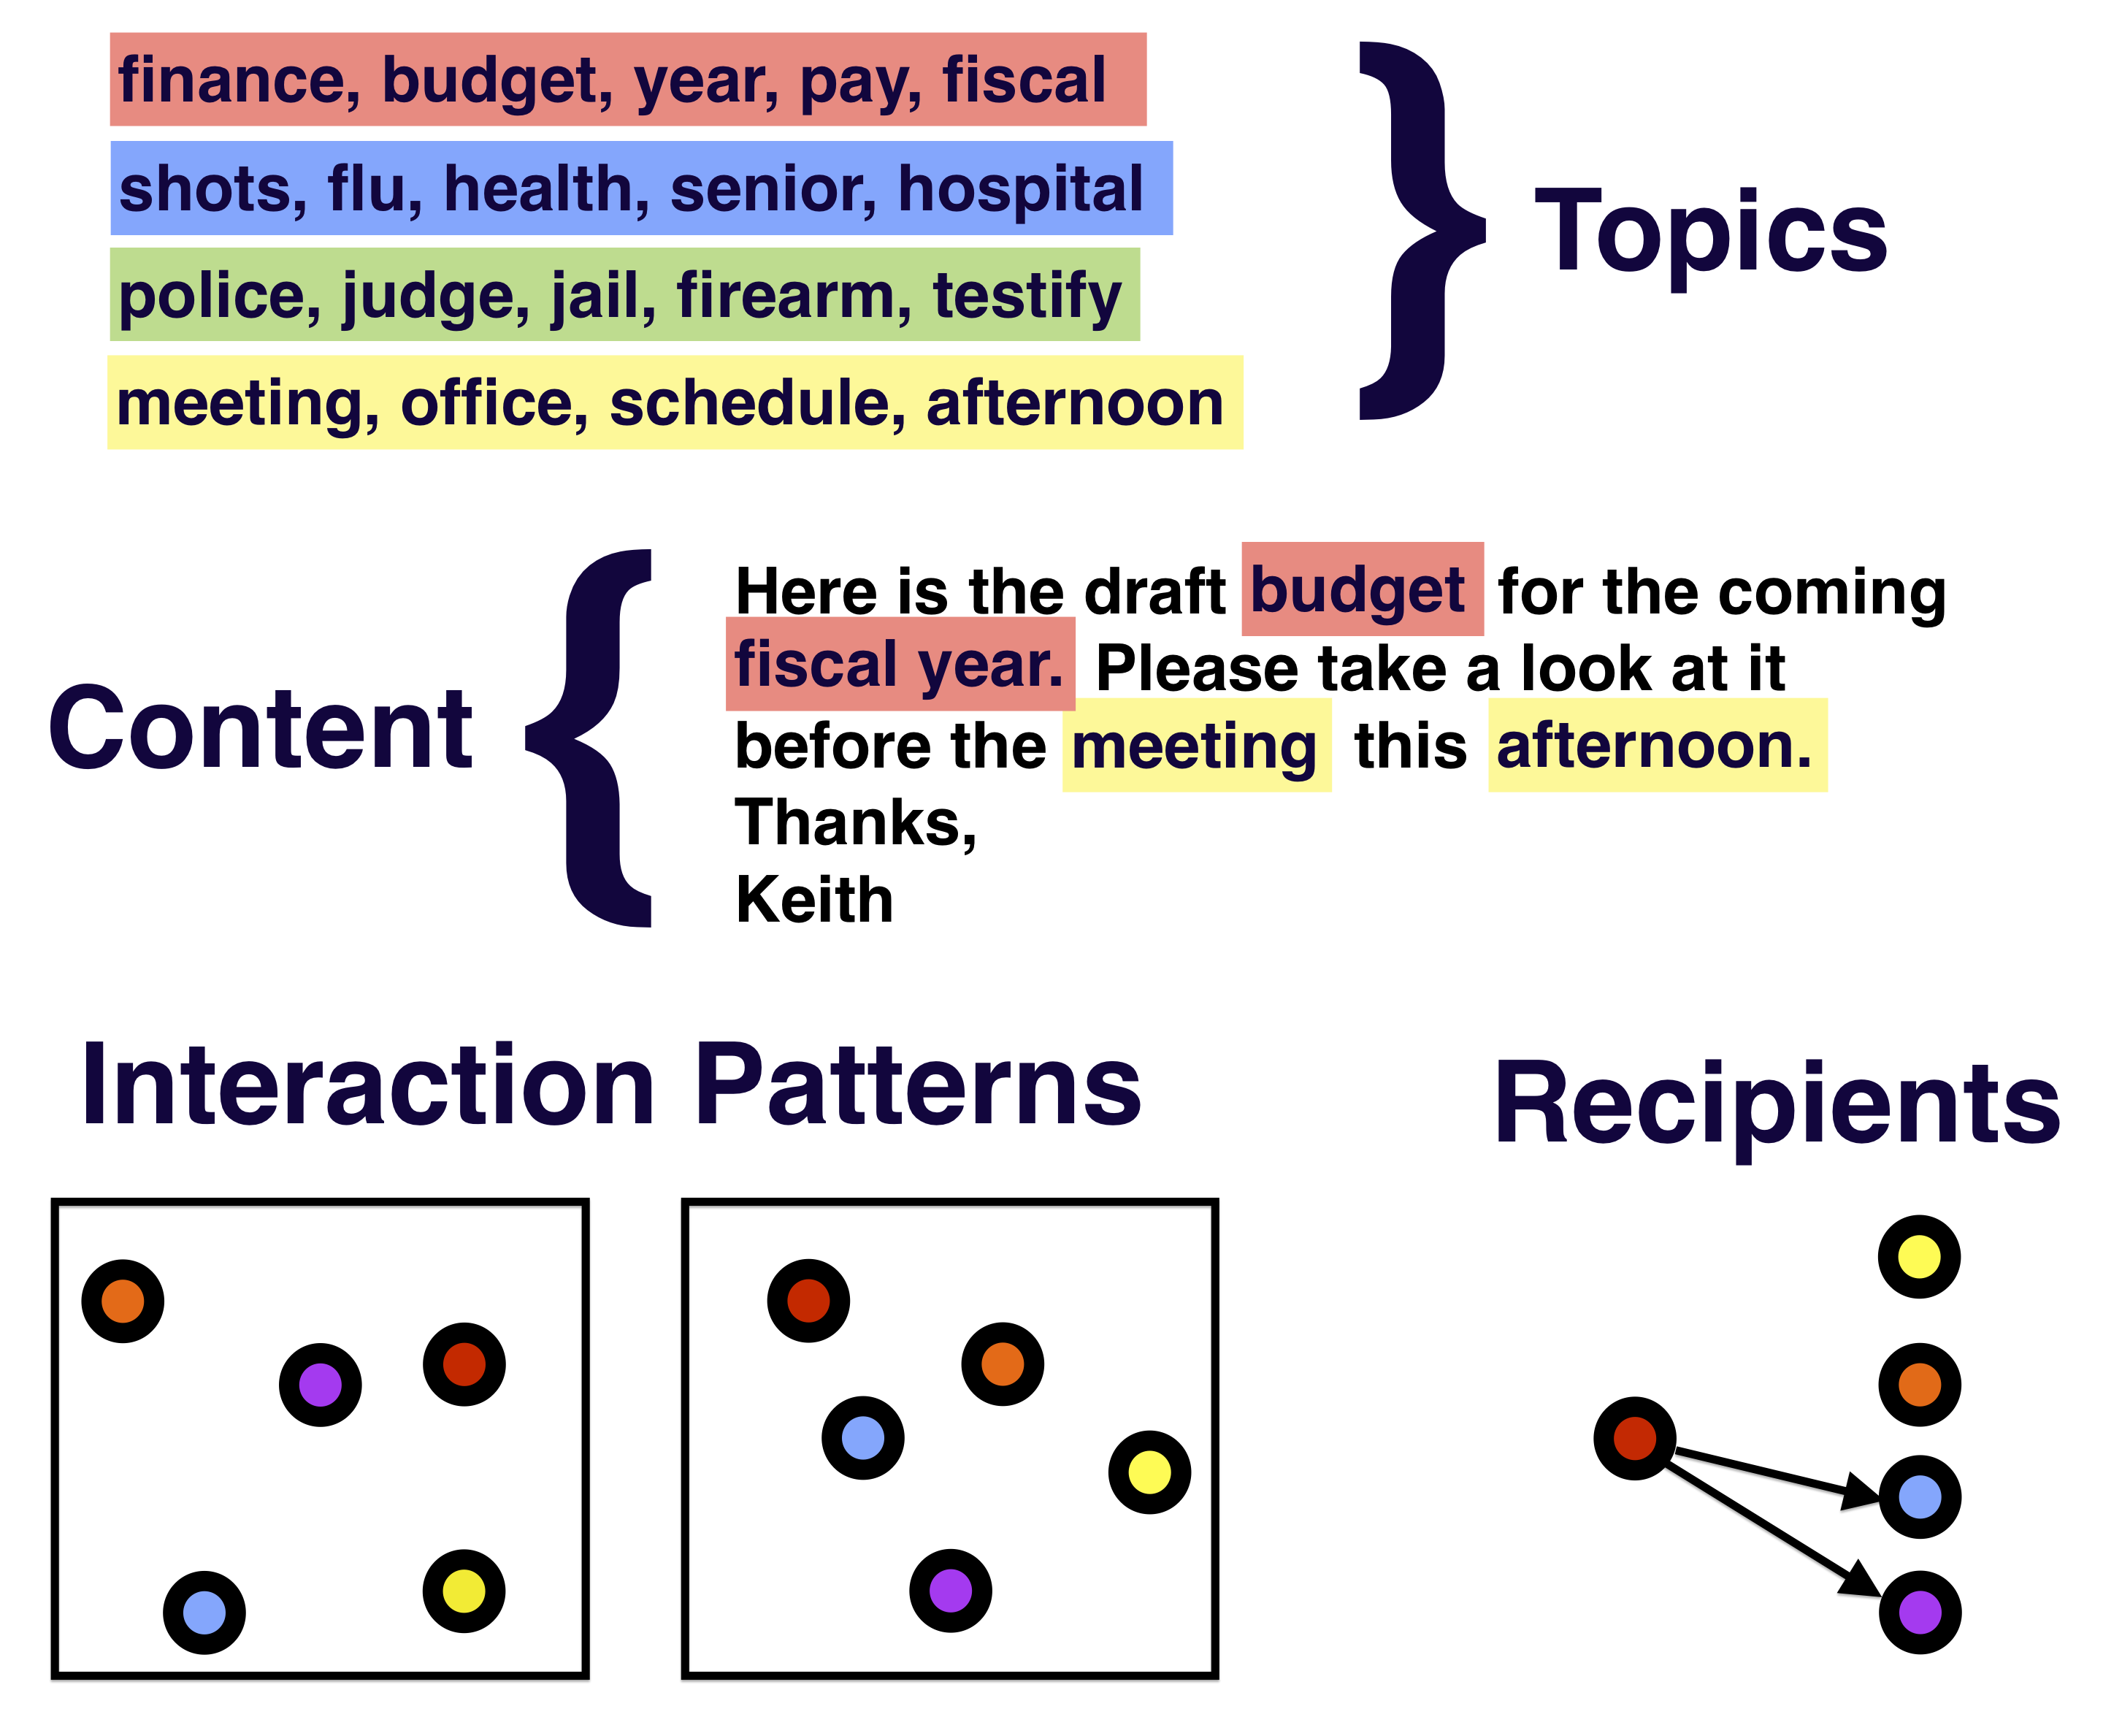
\includegraphics[width=0.98\textwidth]{images/Generative_Process.png}
	\end{changemargin} 
\end{frame}

\begin{frame}\frametitle{Inference}
	\LARGE
	\begin{itemize}
		\item Metropolis within Gibbs sampling.
		\vspace*{.3in}
		\item Separate model for each county.
		\vspace*{.3in}
		\item Include gender mixing covariates.
		\vspace*{.3in}
		\item 40 topics, 4 interaction patterns.
		\vspace*{.3in}
		\item Human code topics used in analysis.
	\end{itemize}
\end{frame}

\begin{frame}\frametitle{Example Model Output}
	
	\centering
	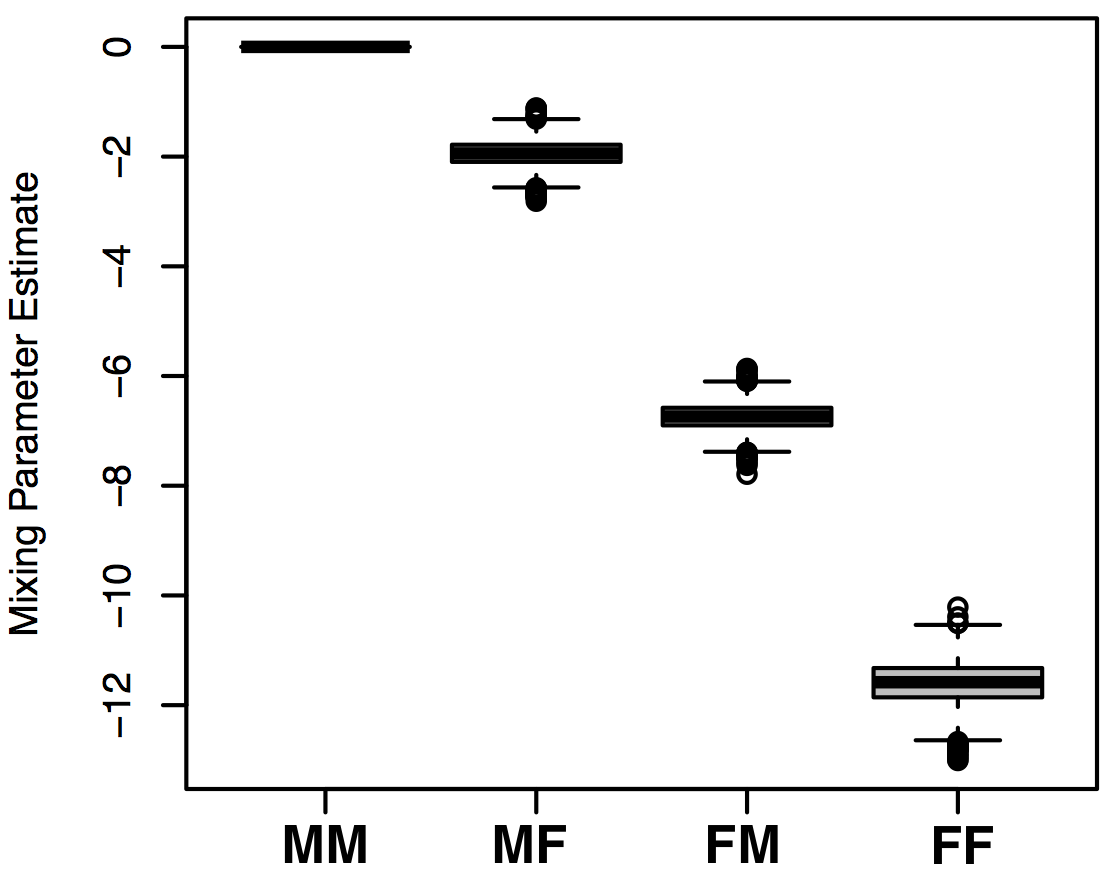
\includegraphics[width = .56\textwidth]{./images/Dare_3_MP.png}\\
	\begin{tabular}{l l}
	\toprule
	Coding & Topic top words\\
	\midrule
	\textbf{Sandy} & will, track, winds, system, forecast\\ 
	\textbf{Sandy} & storm, sandy, high, coastal, tides, night\\ 
	\textbf{Harbor} & status, update, boat, today, weather\\ 
	\textbf{Planning} & board, meeting, planning, seafood, hearing\\ 
	\textbf{Storm} & box, planning, director,  permit, building \\ 
	\bottomrule

	\end{tabular}
	
\end{frame}


\begin{frame}\frametitle{Female-Centric Topics of Communication}
	
	
\begin{changemargin}{-1cm}{ -1cm}	
	\centering
		\begin{tabular}{ll}
			\toprule
	Coding & FF $>$ FM $>$ MF $>$ MM\\
	\midrule

	\textbf{Finance} & order, time, good, april, attached, requests \\ 
	\textbf{Finance} & budget, phone, finance, media, ext, department
	\\ 
	\textbf{Health} & meeting, going, fyi, tricaster, health, project
	 \\ 
	\textbf{Finance} & meeting, box, fax, finance, attached, resolution
	\\ 
	\textbf{Finance} & equity, fax, debt, refunding, time, finance, call
	 \\ 
	\textbf{Finance} & debt, box, fax, finance, policies, contract, audit
	\\ 
	\textbf{Finance} & learn, leader, director, washington, dream
	\\ 
	\textbf{Finance} & fax, ext, phone, finance, director, street
	\\ 
	\textbf{Health} & public, health, email, contact, disclosure

	\\ 
	\textbf{Finance} & good, time, increase, call, pay, office, today
	
	\\ 
	\textbf{Budget} & manager, street, main, fax, office, east, budget
	
	\\ 
	\textbf{Budget} & fund, budget, balance, year, funds, pay, original
	
	\\

			\bottomrule
		\end{tabular}
		\end{changemargin}
\end{frame}


\begin{frame}\frametitle{Male-Centric Topics of Communication}
	
	
\begin{changemargin}{-.9cm}{ -1cm}	
	\centering
		\begin{tabular}{ll}
			\toprule
			Coding & MM $>$ FM $>$ MF $>$ FF\\
			  % & \\
			\midrule

	\textbf{Manager} & office, email, time, staff, meeting, work, good\\ 

	\textbf{IT} & electronic, mail, intended, email, message\\ 

	\textbf{Health} & health, department, project, email, code, garden\\ 


	\textbf{Comments} & jail, mobile, inmates, ago, money, jails\\ 

	\textbf{Planning} & east, planning, street, court, administrator\\ 


	\textbf{Public Works} & public, nashville, suite, washington\\ 


	\textbf{Public Works} & email, energy, carolina, north, address\\ 


	\textbf{Planning} & description, director, street, church, suite\\ 


	\textbf{Planning} & description, fax, phone, director, street, church\\ 


	\textbf{Zoning} & board, meeting, planning, amendment\\ 


	\textbf{Emergency} & operations, emergency, director, lines, street\\ 


	\textbf{Development} & description, director, development, projects\\ 

			\bottomrule
		\end{tabular}
		\end{changemargin}
\end{frame}



\begin{frame}\frametitle{Open Questions, Future Directions}
	\LARGE
	\begin{itemize}
		\item Locus of control. 
		\vspace*{.3in}
		\item Direction of causality.
		\vspace*{.3in}
		\item Interventions to improve gender mixing. 
		\vspace*{.3in}
		\item Cross-organization communication.
	\end{itemize}
\end{frame}

\end{document}
